\documentclass[10pt,a4paper]{scrartcl}

% Note: you must use xelatex to compile this document, as it uses system-font
% MinionPro. Compile by: 'xelatex pili_cv.tex'

\usepackage{array}
\usepackage{fontspec}
\usepackage{wrapfig}
\usepackage{setspace}
\usepackage{scrpage2}
\usepackage{color}
\usepackage[colorlinks=true]{hyperref}
\usepackage[left=3cm,right=3cm,top=3cm,bottom=2.5cm]{geometry}

\pagestyle{scrheadings}
\defaultfontfeatures{Mapping=tex-text}
\setmainfont{Helvetica Light}

\newenvironment{two_col}
{\begin{tabular}{p{2.5cm}p{6.7cm}}}
{\end{tabular}}

\newenvironment{three_col}
{\begin{tabular}{p{6cm}p{5.5cm}>{\hfill}p{1cm}}}
{\end{tabular}}

\newenvironment{four_col}
{\begin{tabular}{p{4.5cm}p{2cm}p{2.4cm}p{3.0cm}}}
{\end{tabular}}

% Appearance
\makeatletter
\renewcommand\section{%
  \@startsection{section}{1}%
  {0pt}%
  {-3.5ex \@plus -1ex \@minus -.2ex}%
  {2.5ex \@plus.2ex}%
  {\normalfont\Large\bfseries\color[rgb]{0.0, 0.2, 0.5}}}
\renewcommand\subsection{%
  \@startsection{section}{2}%
  {0pt}%
  {-3.5ex \@plus -1ex \@minus -.2ex}%
  {2.3ex \@plus.2ex}%
  {\normalfont\bfseries\color[rgb]{0.0, 0.0, 0.0}}}
\makeatother

\newcommand\sometitle[1]{{\Huge #1}}
\newcommand\explanation[1]{\color[rgb]{0.5, 0.5, 0.5}\textit{#1}}
\setlength\parindent{0pt}
\setlength\parskip{8pt}




% FOOTER
\cfoot{\normalfont Pilar Andrea Quiroz Pardo \quad \textbar \quad pili.a.quiroz@gmail.com}

\begin{document}

{\fontspec{DejaVu Sans} \sometitle{Pilar Andrea Quiroz}}
\\
\onehalfspacing
\normalsize

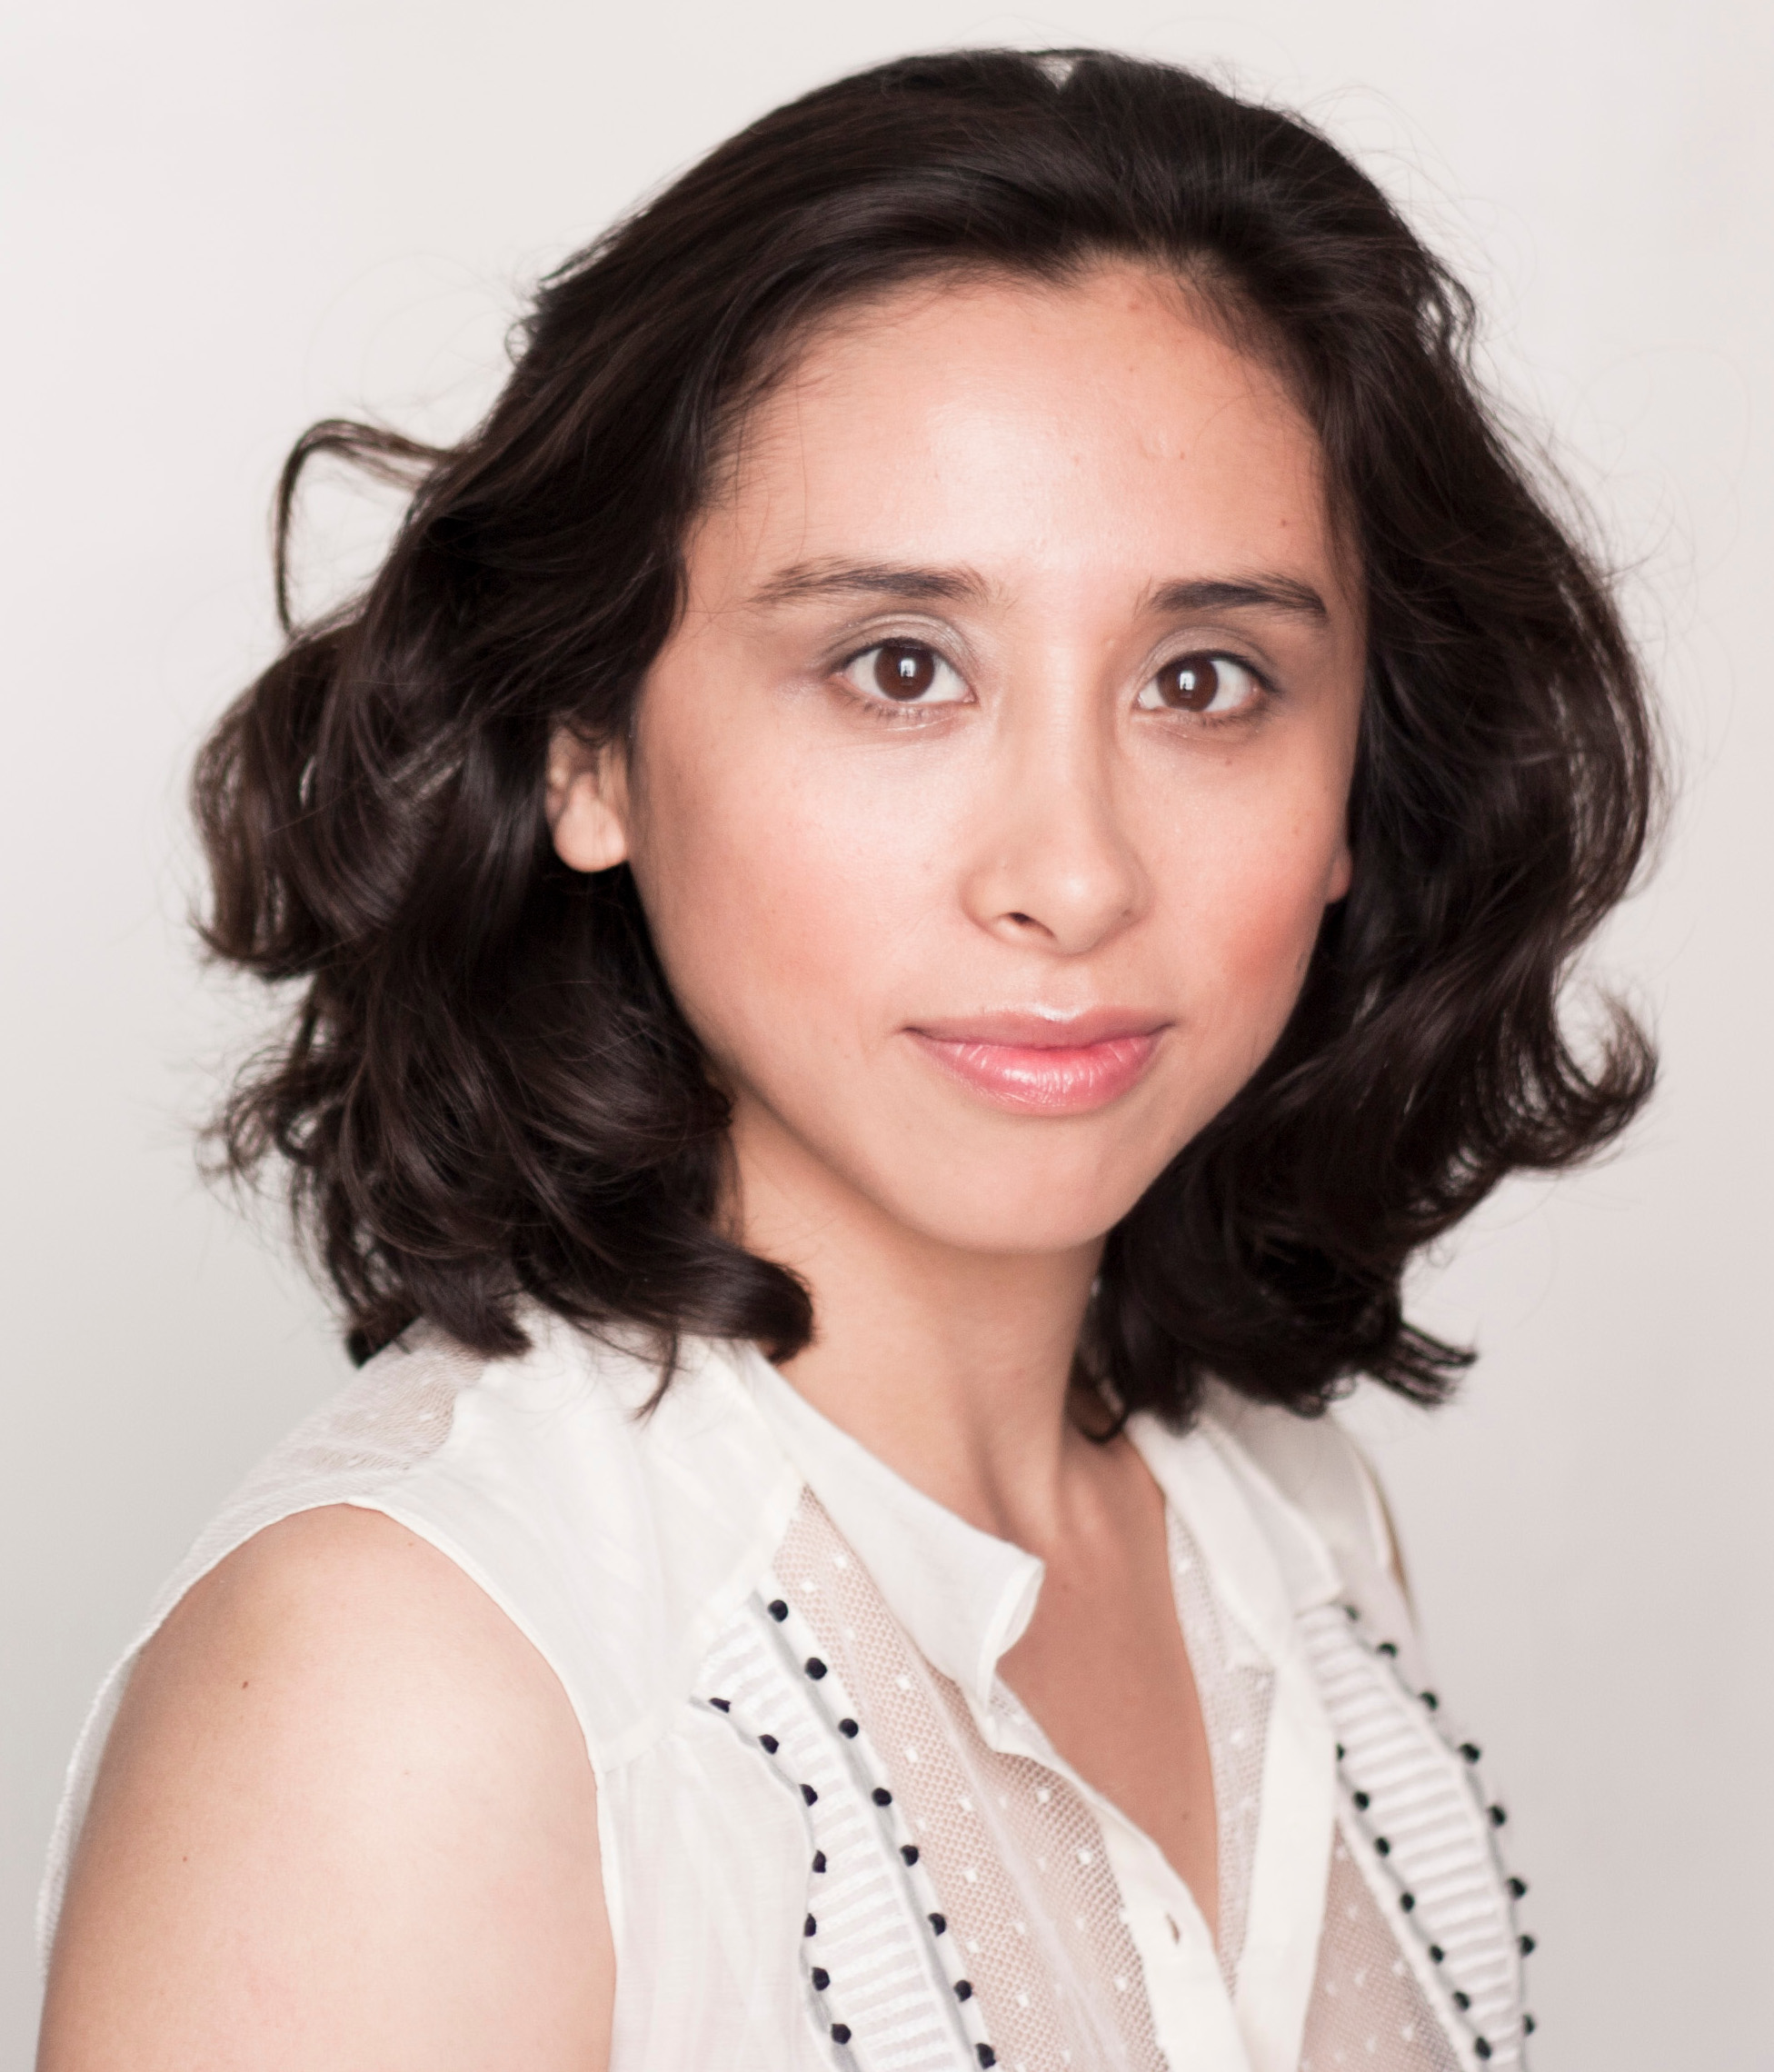
\includegraphics[width=0.6\textwidth]{pili_big3.jpg}
\\
\\




Pilar Andrea Quiroz is an international theatre performer currently based in
Germany. Originally from Colombia, she moved to Paris to study theatre at Ecole
Jacques Lecoq. After one year there, she went on to graduate from the 2 year
program at Ecole Philippe Gaulier.

Pilar is also one of the founding members and administrators of the Cultural
Association Trastorno Obsesivo Teatral, a theatre group in Bogota, and Ubuntu,
a group of actors, artists, and acrobats that create physical theatre using
dance and acrobatics to explore the human body as a metaphor for conflict and
balance.


\end{document}
